\documentclass{article}
\usepackage{amsmath}
\usepackage{graphicx}
\usepackage[x11names,svgnames,dvipsnames]{xcolor}
\usepackage{tcolorbox}
\usepackage{pgfplots}
\usepackage{amssymb}
\usetikzlibrary{arrows.meta}

% Define custom colors
\definecolor{myblue}{RGB}{70,130,180}

% Create a box style for highlights
\tcbset{
    mybox/.style={
        colframe=myblue,
        colback=white,
        sharp corners,
        boxrule=1pt,
        left=0pt,
        right=0pt,
        top=0pt,
        bottom=0pt
    }
}

\title{Periodic Functions}
\author{Kensukeken}
\date{January 18, 2024}

\begin{document}

\maketitle

\section{Introduction}

\begin{tcolorbox}[mybox]
Sinusoidal function are periodic function where graph looks like smooth symmetical waves, where any potion can be horizontally translated onto another potion of curve. \\
Graph of sinusdidal function can be created by transforming $y=\sin{\theta}$ and $y=\cos{\theta}$.\\

    A periodic function is a function that repeats its values in regular intervals. In this document, we will explore the properties and examples of periodic functions.\\
    Note: sinusoidal function are all period function but period function are not sinusoidal.
    
\end{tcolorbox}

\begin{center}
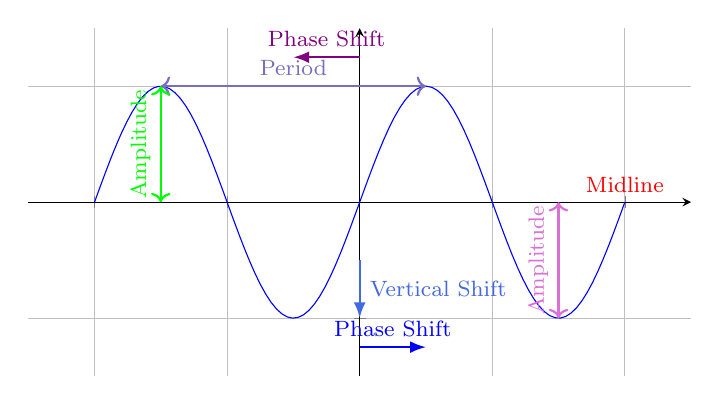
\begin{tikzpicture}
\begin{axis}[
    axis lines=middle,
    xticklabels={},
    yticklabels={},
    xtick={-2*pi,-pi,0,pi,2*pi},
    ytick={-2,0,2},
    grid=major,
    ymin=-3,
    ymax=3,
    xmin=-2.5*pi,
    xmax=2.5*pi,
    width=10cm,
    height=6cm
]
\addplot[domain=-2*pi:2*pi, samples=100, color=blue]{2*sin(deg(x))};
\draw[dashed] (axis cs:-2*pi,0)--(axis cs:2*pi,0);
\node[align=center, font=\footnotesize, color=red] at (axis cs:2*pi,0.3){Midline};
\draw[<->, Periwinkle, thick] (axis cs:pi/2,2.0)--(axis cs:-3*pi/2,2.0) node[midway,above,font=\footnotesize]{Period};
\draw[<->, green, thick] (axis cs:-1.5*pi,0)--(axis cs:-1.5*pi,2) node[midway,left,font=\footnotesize,rotate=90,above]{Amplitude};
\draw[<->, Orchid, thick] (axis cs:1.5*pi,-2)--(axis cs:1.5*pi,0) node[midway,right,font=\footnotesize,rotate=-270,above]{Amplitude};
\draw[-{Latex[length=2mm]}, Purple, thick] (axis cs:0,2.5)--(axis cs:-pi/2,2.5) node[midway,above,font=\footnotesize]{Phase Shift};
\draw[-{Latex[length=2mm]}, blue, thick] (axis cs:0,-2.5)--(axis cs:pi/2,-2.5) node[midway,above,font=\footnotesize]{Phase Shift};
\draw[-{Latex[length=2mm]}, RoyalBlue, thick] (axis cs:0,-1)--(axis cs:0,-2) node[midway,right,font=\footnotesize]{Vertical Shift};
\end{axis}
\end{tikzpicture}
\end{center}


Midline, amplitude, and period are three features of sinusoidal graphs.
\newpage
\section{Characteristics of Sinusoidal Graphs}
\subsection{Midline/Axis of the Curve:}
The \textcolor{Maroon}{\underline{midline}} is a horizontal line right in the middle between the highest and lowest points of the graph. It's calculated using the formula:
\[y = \frac{\text{max value + min value}}{2}\]

\subsection{Amplitude:}
The \textcolor{LimeGreen}{\underline{amplitude}} is how high or low the graph reaches from the middle line. You find it using:
\[a = \frac{\text{max value - min value}}{2}\]

\subsection{Period:}
The \textcolor{Periwinkle}{\underline{period}} is how wide one complete cycle of the graph is. It's found by looking at the distance between two consecutive high or low points. The formula is:
\[P = \frac{2\pi}{k}\quad \text{or} \quad P = \frac{360}{k} \]

\subsection{Phase Shift:}
The \textcolor{Purple}{\underline{phase shift}} is like a sideways movement of the graph, showing if it's shifted left or right. For \(y = A \sin(k \theta + d) + C\), you calculate it using:
\[\text{Horizontal shift} = \frac{d}{k} \text{ or }  -\frac{d}{k}\]

\subsection{Vertical Shift:}
The \textcolor{RoyalBlue}{\underline{vertical shift}} is like lifting or lowering the whole graph. For \(y = A \sin(k \theta + d) + C\), it shifts the entire graph up or down by \(C\) units.

\subsection{Key Intervals:}
\textcolor{OliveGreen}{\underline{Key intervals}} are specific ranges of values where the graph undergoes significant changes. These intervals are essential for identifying crucial points, such as the highest and lowest values, contributing to a better understanding of the function's behavior.

One important key interval is $\frac{\text{Period}}{4}$, representing a quarter of the period. It marks a position in the graph where distinctive shifts and changes occur, aiding in the analysis of the function's characteristics.

\section{Trigonometric Functions}
The graphs of $y=\sin\theta, y=\cos\theta, y=\tan\theta.$ are shown below.
\begin{figure}[h]
    \centering
    \includegraphics[width=1.0\textwidth]{Unit 6/sin-cos-tan.png}
\end{figure}
\section{Transformations of Trigonometric Functions}
\begin{itemize}
    \item Transformations apply to trig functions as they do to any other function.
    \item The graphs of $y=a \sin k(\theta+d)+c$ and $y=a \cos k(\theta+b)+d$ are transformations of the graphs $y=\sin \theta$ and $y=\cos \theta$ respectively.
    \item The value of $a$ determines the vertical stretch, called the amplitude. It also tells whether the curve is reflected in the $\theta$-axis.
    \item The value of $k$ determines the horizontal stretch. The graph is stretched by a factor of $\frac{1}{k}$. We can use this value to determine the period of the transformation of $y=\sin \theta$ or $y=\cos \theta$.
    \item The period of $y=\sin k \theta$ or $y=\cos k \theta$ is $\frac{360^{\circ}}{k}, k>0$. The period of $y=\tan k \theta$ is $\frac{180^{\circ}}{k}, k>0$.
    \item The value of $d$ determines the horizontal translation, known as the phase shift.
    \item The value of $\mathrm{c}$ determines the vertical translation. $y=d$ is the equation of the axis of the curve.
\end{itemize}

\section*{Examples}
\begin{itemize}
    \item 
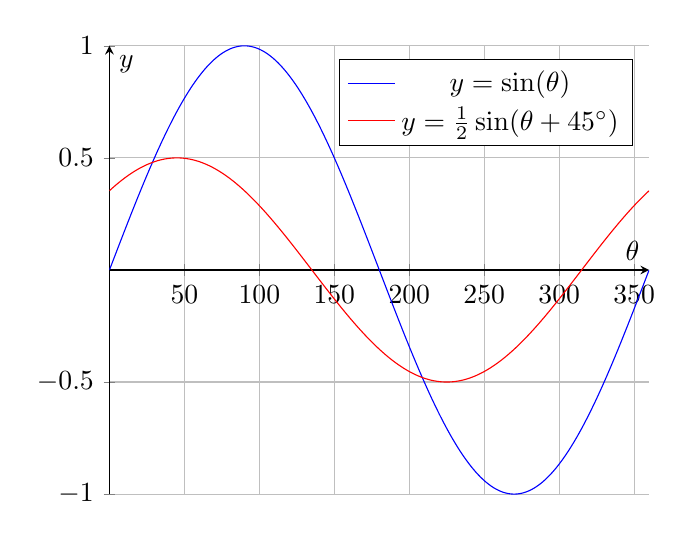
\begin{tikzpicture}
    \begin{axis}[
        domain=0:360, % Assuming you want to plot over one full revolution (0 to 360 degrees)
        samples=500, % Number of samples for a smooth curve
        xlabel={$\theta$},
        ylabel={$y$},
        legend pos=north east,
        grid=both,
        axis lines=middle
    ]

    % Plot y = sin(theta) and y = 0.5*sin(theta + 45)
    \addplot[blue, smooth] {sin(x)};
    \addlegendentry{$y = \sin(\theta)$}

    \addplot[red, smooth] {0.5*sin(x + 45)};
    \addlegendentry{$y = \frac{1}{2}\sin(\theta + 45^\circ)$}

    \end{axis}
\end{tikzpicture}
\item 
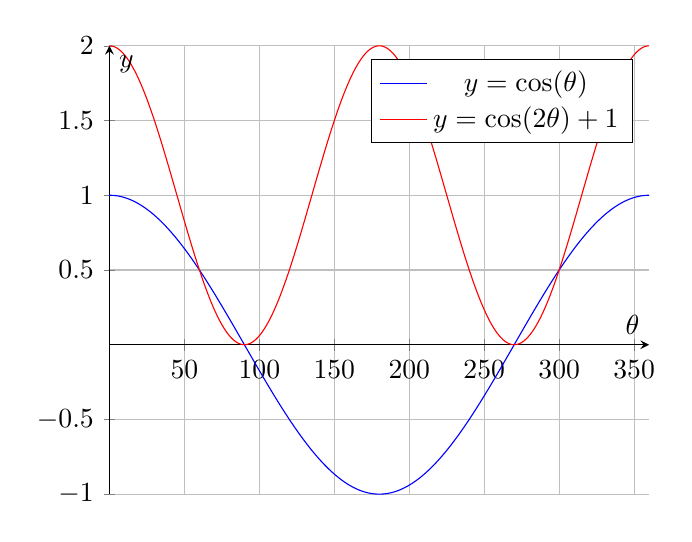
\begin{tikzpicture}
    \begin{axis}[
        domain=0:360, % Assuming you want to plot over one full revolution (0 to 360 degrees)
        samples=500, % Number of samples for a smooth curve
        xlabel={$\theta$},
        ylabel={$y$},
        legend pos=north east,
        grid=both,
        axis lines=middle
    ]

    % Plot y = cos(theta) and y = cos(2*theta) + 1
    \addplot[blue, smooth] {cos(x)};
    \addlegendentry{$y = \cos(\theta)$}

    \addplot[red, smooth] {cos(2*x) + 1};
    \addlegendentry{$y = \cos(2\theta) + 1$}

    \end{axis}
\end{tikzpicture}
\end{itemize}
\newpage
\subsection{Property of Sine function }
\begin{tabular}{|c|c|}
\hline
\textbf{Property} & \(y = \sin(x)\) \\
\hline
Amplitude & 1 \\
\hline
Period & \(360^\circ\) \\
\hline
Equation of Axis & \(y = 0\) \\
\hline
Domain & \(\{x | x \in \mathbb{R}\}\) \\
\hline
Range & \(\{y \in \mathbb{R} | -1 \leq y \leq 1\}\) \\
\hline
x-intercepts & \(x \in \{180n, n \in \mathbb{Z}\}\) \\
\hline
y-intercept & 0 \\
\hline
Maximum & \(1, \text{when } x \in \{90 + 360n, n \in \mathbb{Z}\}\) \\
\hline
Minimum & \(-1, \text{when } x \in \{270 + 360n, n \in \mathbb{Z}\}\) \\
\hline
Intervals of increase & \(90 < x < 270, \text{and all intervals obtained by adding } 360n, n \in \mathbb{Z}\) \\
\hline
Intervals of decrease & \(270 < x < 90, \text{and all intervals obtained by adding } 360n, n \in \mathbb{Z}\) \\
\hline
\end{tabular}

\subsection{Property of Cosine function}
\begin{tabular}{|c|c|}
\hline
\textbf{Property} & \(y = \cos(x)\) \\
\hline
Amplitude & 1 \\
\hline
Period & \(360^\circ\) \\
\hline
Equation of Axis & \(y = 0\) \\
\hline
Domain & \(\{x | x \in \mathbb{R}\}\) \\
\hline
Range & \(\{y \in \mathbb{R} | -1 \leq y \leq 1\}\) \\
\hline
x-intercepts & \(x \in \{90 + 180n, n \in \mathbb{Z}\}\) \\
\hline
y-intercept & 1 \\
\hline
Maximum & \(1, \text{when } x \in \{360n, n \in \mathbb{Z}\}\) \\
\hline
Minimum & \(-1, \text{when } x \in \{180 + 360n, n \in \mathbb{Z}\}\) \\
\hline
Intervals of increase & \(0 < x < 180, \text{and all intervals obtained by adding } 360n, n \in \mathbb{Z}\) \\
\hline
Intervals of decrease & \(180 < x < 360, \text{and all intervals obtained by adding } 360n, n \in \mathbb{Z}\) \\
\hline
\end{tabular}
\newpage


\newpage
% Extras
\section{Extra}
\subsection{Definition}

A function $f(x)$ is periodic with period $T$ if, for all $x$ in the domain of $f$, the following holds:

\[
f(x + T) = f(x)
\]

This means that the function values repeat every $T$ units along the $x$-axis.

\subsection{Examples}

\subsubsection{Sine Function}

\begin{tcolorbox}[mybox]
    The sine function, denoted by $\sin(x)$, is a classic example of a periodic function. Its period is $2\pi$, and the function is defined as:
    
    \[
    \sin(x) = \sum_{n=0}^{\infty} \frac{(-1)^n}{(2n+1)!} x^{2n+1}
    \]
\end{tcolorbox}

\begin{figure}[h]
    \centering
    \includegraphics[width=0.6\textwidth]{Unit 6/Sine-Graph.png}
    \caption{Graph of the sine function.}
\end{figure}
\newpage 
\subsubsection{Square Wave}

\begin{tcolorbox}[mybox]
    The square wave is another example of a periodic function. It has a period $T$ and is defined as:
    
    \[
    \text{square wave}(x) = 
    \begin{cases} 
    1 & \text{if } 0 \leq x < \frac{T}{2} \\
    -1 & \text{if } \frac{T}{2} \leq x < T
    \end{cases}
    \]
\end{tcolorbox}

\begin{figure}[h]
    \centering
    \includegraphics[width=0.6\textwidth]{Unit 6/square_wave.JPG}
    \caption{Graph of a square wave.}
\end{figure}

\section{Conclusion}

\begin{tcolorbox}[mybox]
    Periodic functions are essential in various branches of mathematics and physics. Understanding their properties and behavior is crucial for analyzing and modeling periodic phenomena.
\end{tcolorbox}
\usetikzlibrary{3d, shapes.multipart}
\tikzset{>=latex} 
\tikzset{axis/.style={black, thick,->}}
\tikzset{vector/.style={>=stealth,->}}
\tikzset{every text node part/.style={align=center}}
\begin{tikzpicture}[x={(-150:0.7)}, y={(90:1.0)}, z={(-15:8mm)}]
\def\wave{
    \draw[fill, very thick, fill opacity=.2]
         (0,0) sin (1,1) cos (2,0) sin (3,-1) cos (4,0)
               sin (5,1) cos (6,0) sin (7,-1) cos (8,0)
               sin (9,1) cos (10,0) sin (11,-1) cos (12,0);
         
    \foreach \shift in {0,4,8}
    {
        \begin{scope}[xshift=\shift cm,thin]
                \draw[-stealth, thick] (.5,0)  -- (0.5,0 |- 45:1cm);
                \draw[-stealth, thick] (1,0)   -- (1,1);
                \draw[-stealth, thick] (1.5,0) -- (1.5,0 |- 45:1cm);
                \draw[-stealth, thick] (2.5,0) -- (2.5,0 |- -45:1cm);
                \draw[-stealth, thick] (3,0)   -- (3,-1);
                \draw[-stealth, thick] (3.5,0) -- (3.5,0 |- -45:1cm);
         \end{scope}
    } 
}
\begin{scope}[canvas is zy plane at x=0, draw=red, fill=red] 
    \draw[-latex, thick, black] (0,0) -- (0, 1.5) node[above] {$\mathbf E$};
    \wave
\end{scope}
\begin{scope}[canvas is zx plane at y=0, draw=blue, fill=blue]
    %% Direction of Propagation
    \draw[-latex, thick, black] (0,0) -- (12.5, 0) node[rotate = -12, pos=1.1] {Propagation\\Direction};
    \draw[-latex, thick, black] (0,0) -- (0,2) node[left] {$\mathbf B$};
    \wave
\end{scope}
\end{tikzpicture}
\end{document}

